\section{稳健性检验}

\subsection{标签阈值稳健性}

首先，本文检验压力标签阈值是否影响核心预警结论。基准设定使用训练期 90\% 分位数定义压力事件，稳健性检验进一步考察 85\% 和 95\% 分位阈值。阈值降低会提高事件发生率，阈值提高会使压力事件更稀有；如果模型仅依赖某一固定阈值，则 PR-AUC、Top 5\% 命中率和 lift 应出现明显不稳定。

图 \ref{fig:robust-label} 展示标签阈值变化下的 SMARTBoost 样本外预警表现。

\begin{figure}[H]
    \centering
    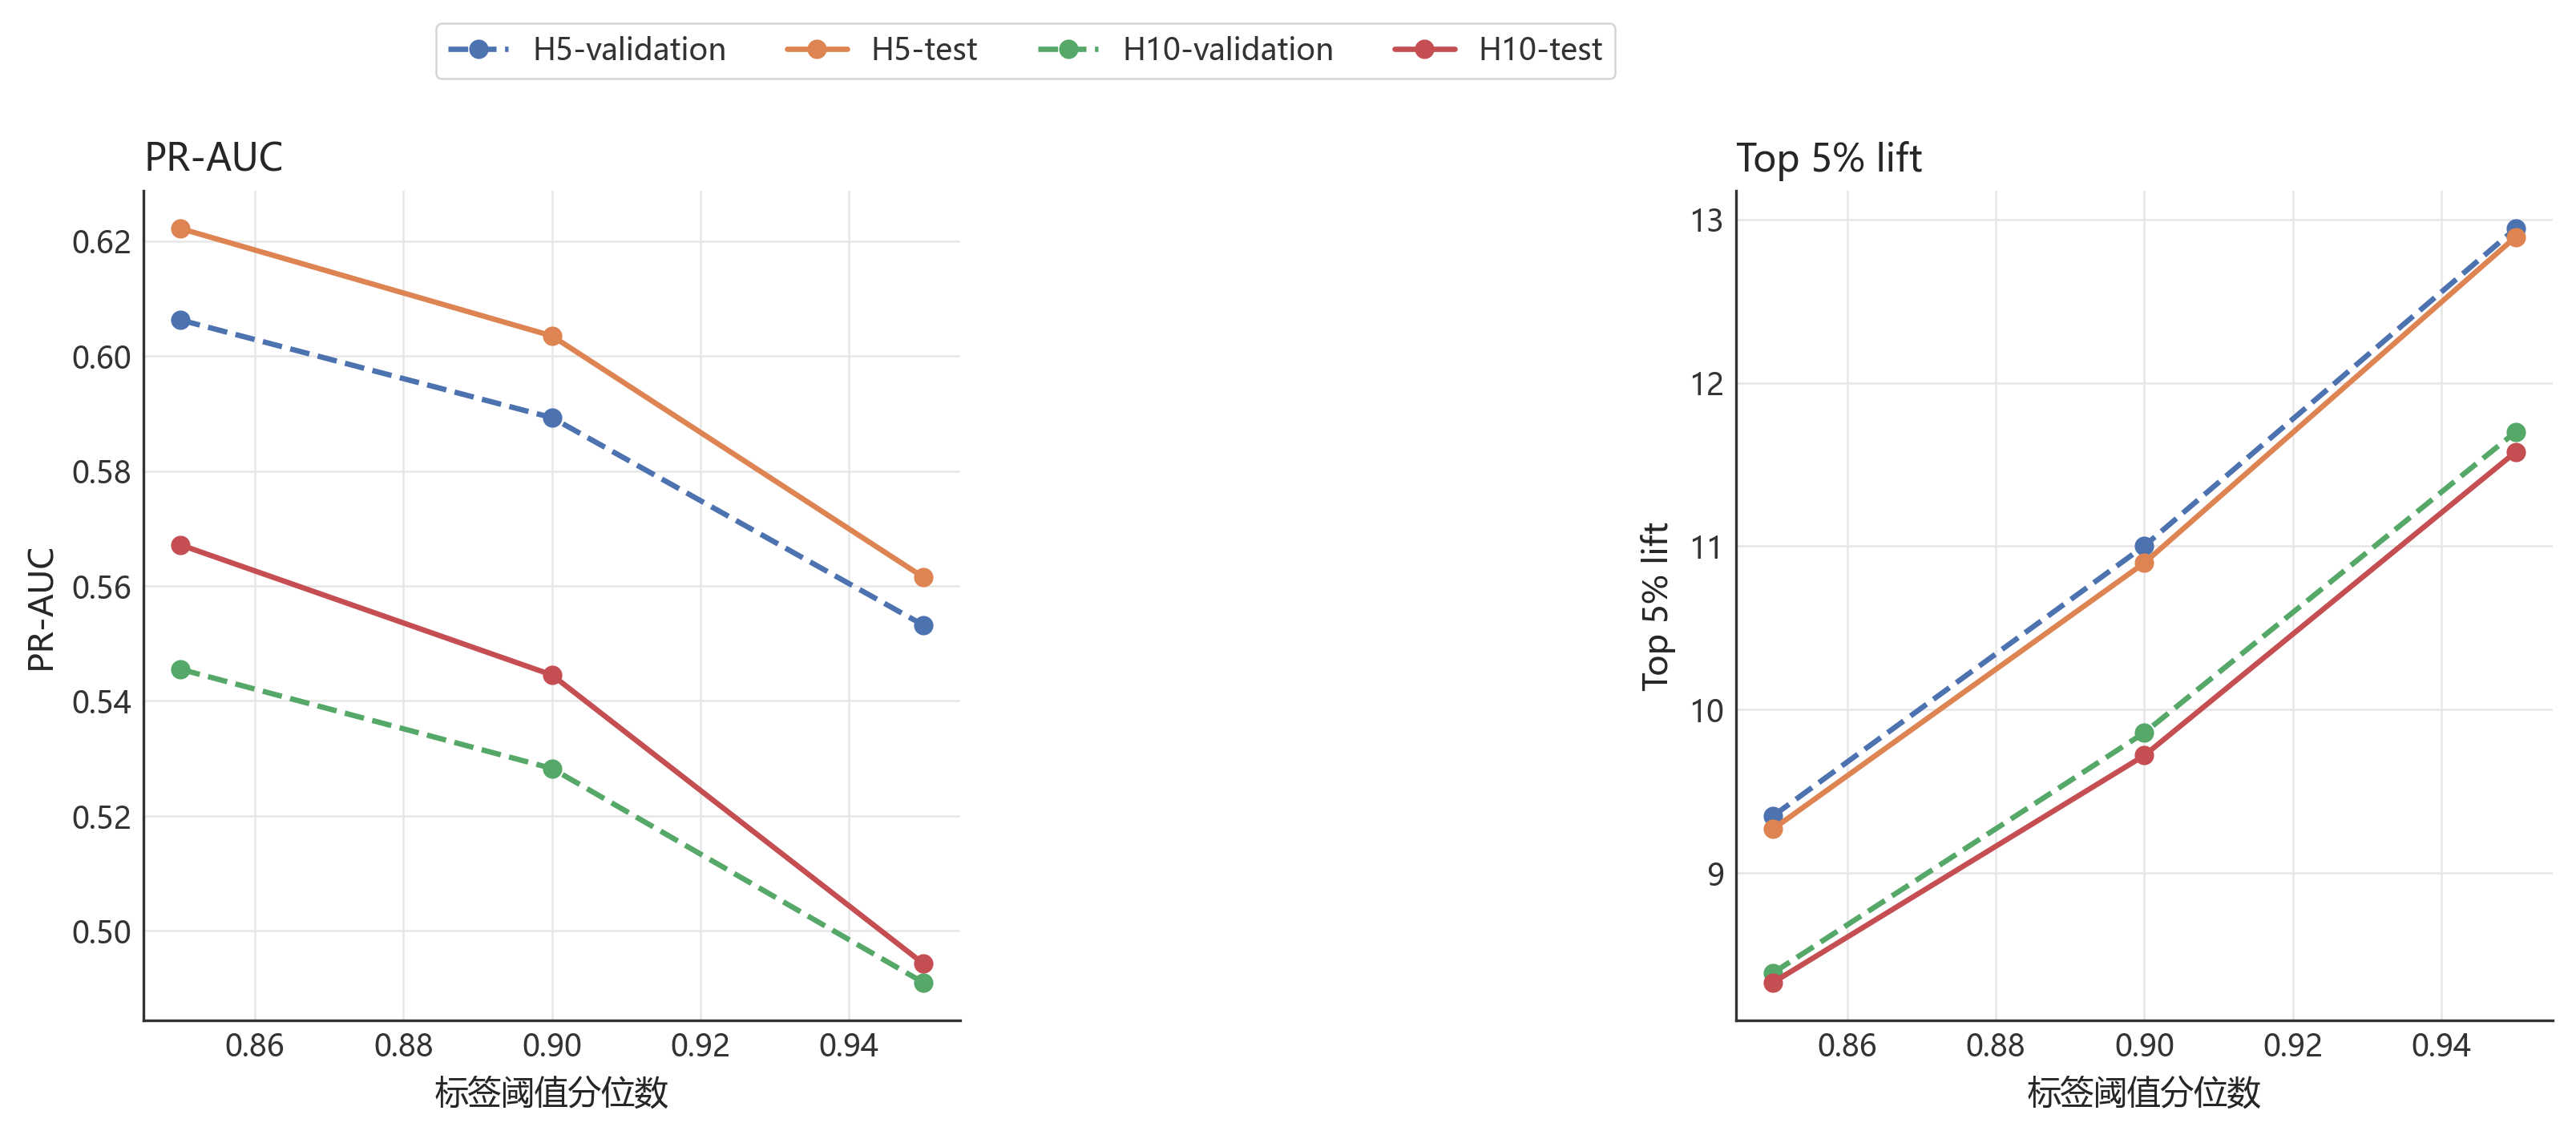
\includegraphics[width=0.90\textwidth]{figures/fig_robust_label_threshold.png}
    \caption{标签阈值变化下的 SMARTBoost 样本外预警表现。图中比较不同训练期分位阈值下的事件率、PR-AUC 与高风险组 lift。}
    \label{fig:robust-label}
\end{figure}

图 \ref{fig:robust-label} 显示，虽然不同阈值下的事件基准率和 PR-AUC 水平存在差异，但高风险组相对于基准事件率的 lift 提升方向保持一致。Top 5\% 组始终捕捉到比平均水平更高的压力集中度，说明模型的核心排序结论保持一致，而不是完全依赖某一固定标签阈值。阈值变化会同步改变事件率和 PR-AUC 绝对水平，因此评价重点应放在 lift 与排序方向能否跨阈值保持稳定，而非绝对指标数值的横向比较。

\subsection{RGARCH realized pressure measure 稳健性}

RGARCH-CARR-SK 的稳健性主要体现在 realized pressure measure 的替代设定上。正文表 \ref{tab:rgarch-loss} 已经比较 RV、RBV、MedRV 与 RMAD 四类测度的样本外损失。不同测度下的损失差异说明，条件压力风险路径对测度口径具有敏感性。

图 \ref{fig:rgarch-realized-dist} 展示不同 realized pressure measure 的标准化分布差异。

\begin{figure}[H]
    \centering
    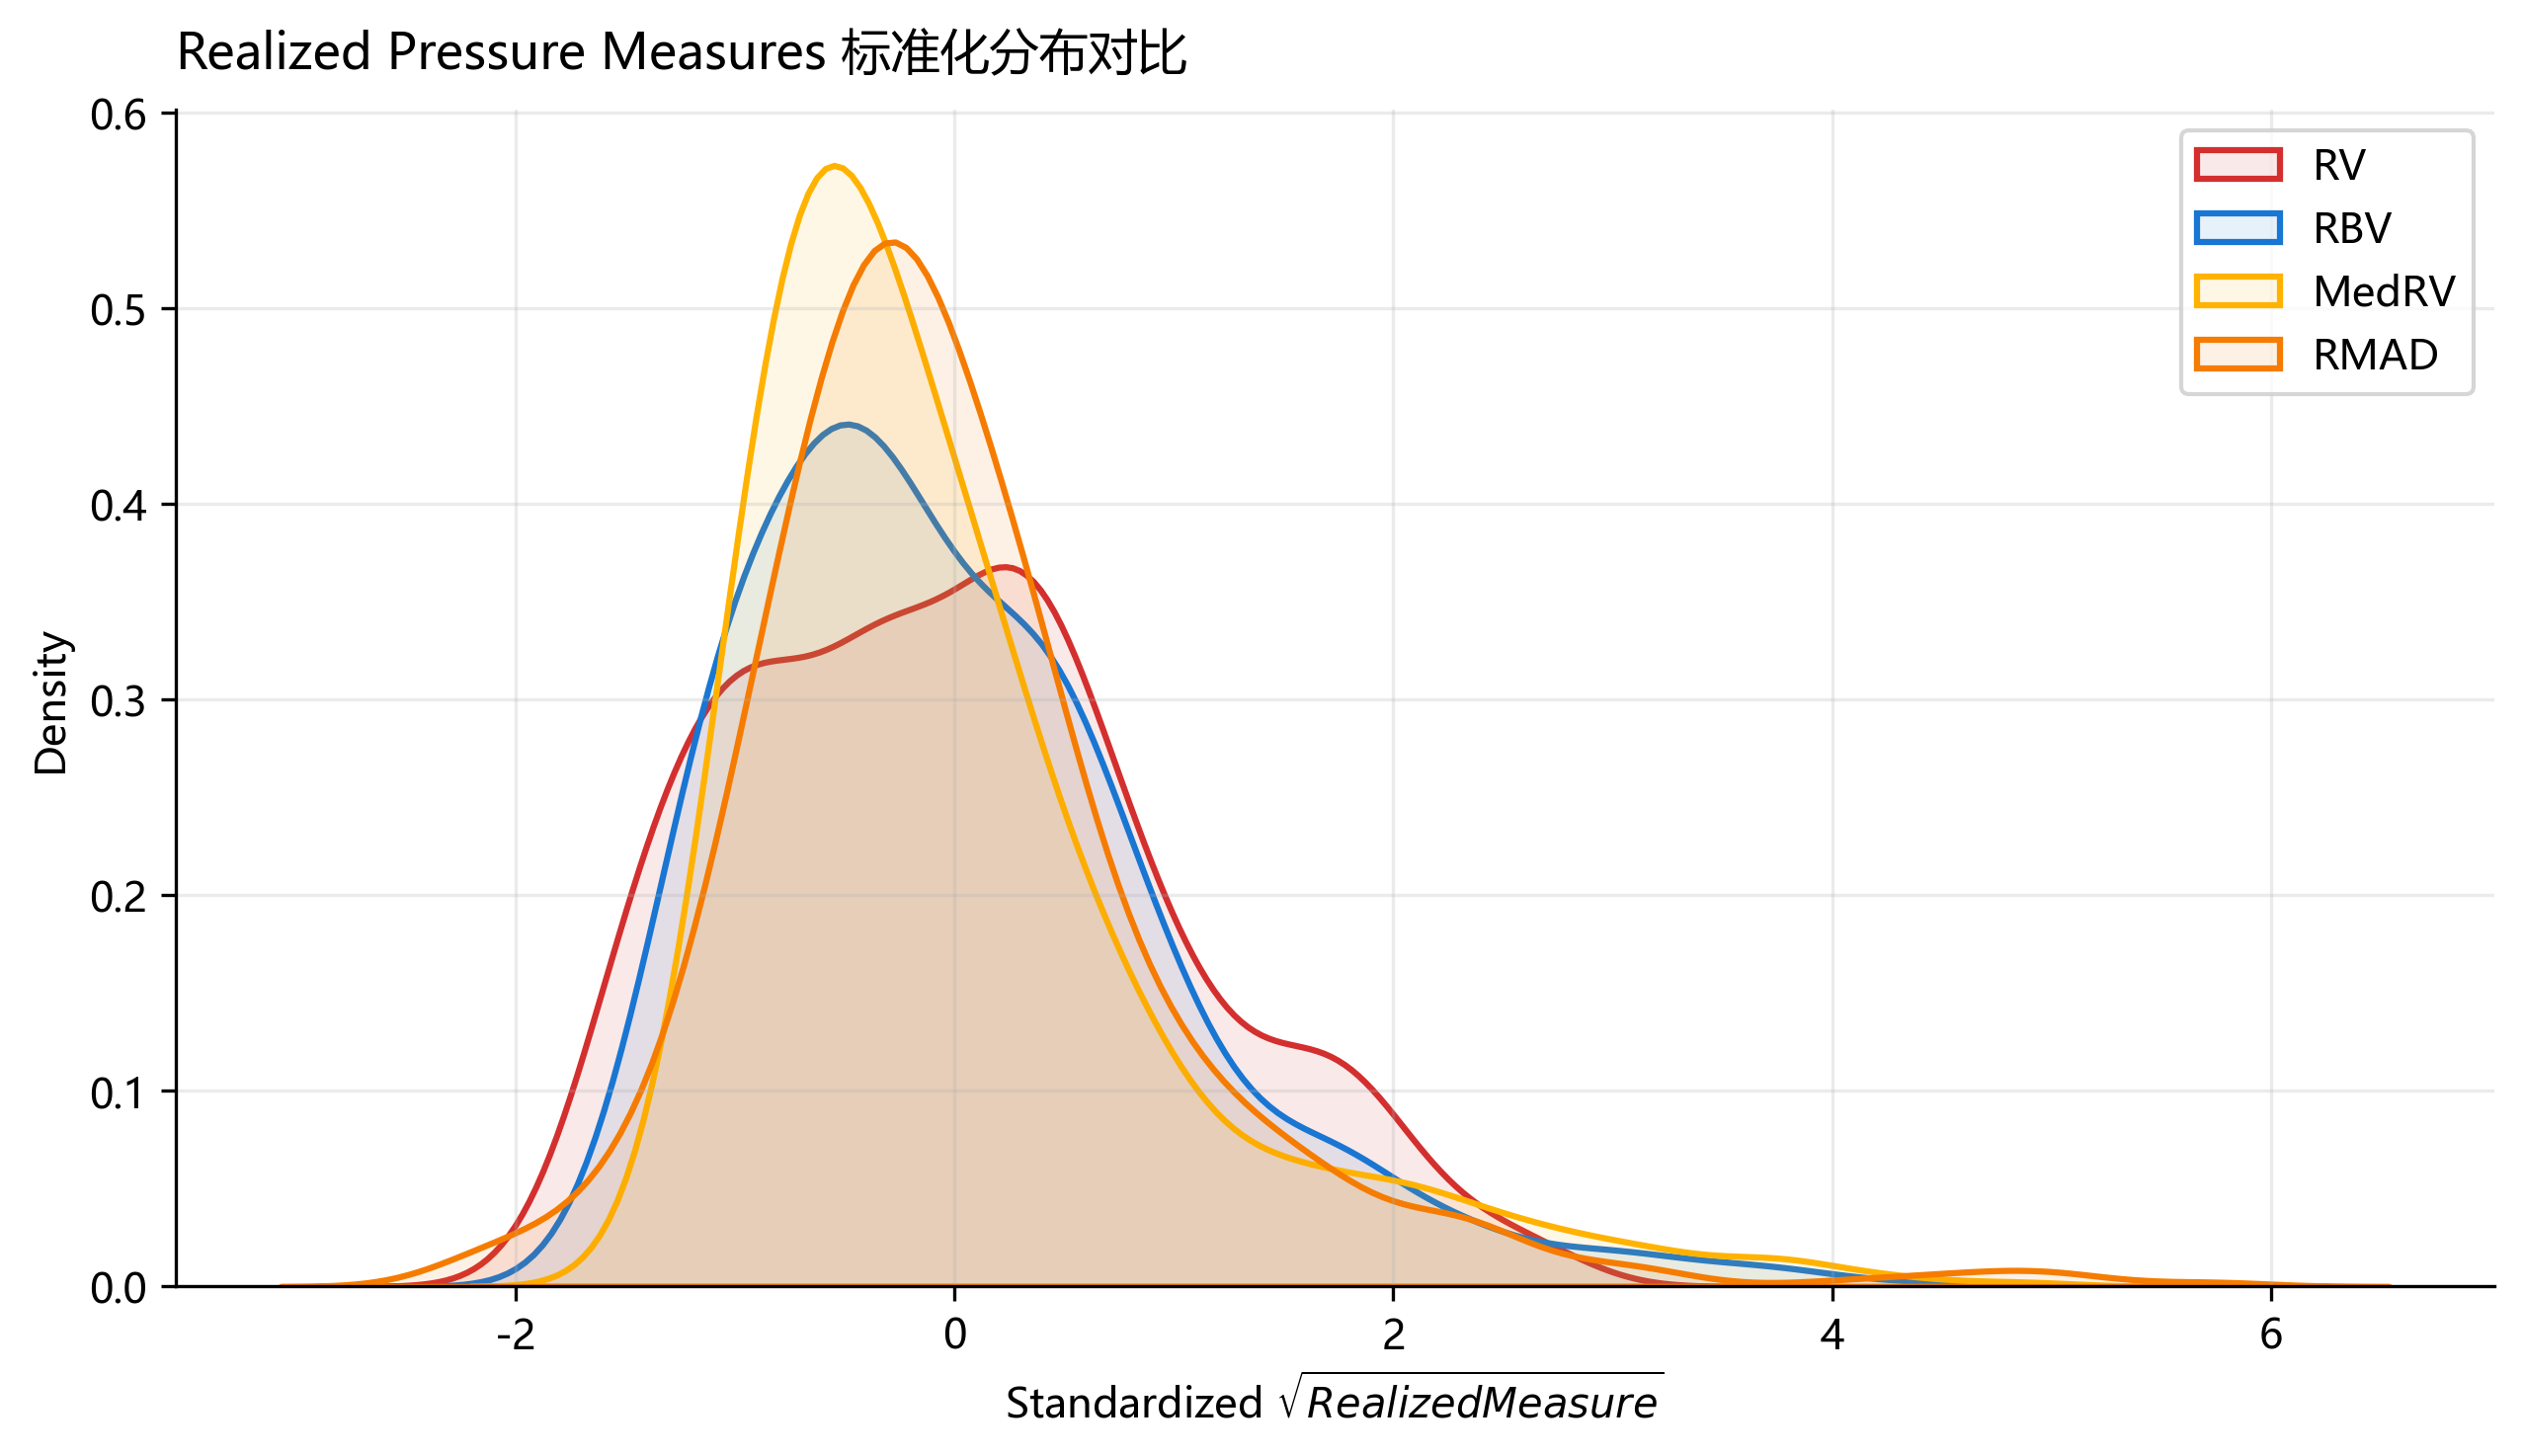
\includegraphics[width=0.86\textwidth]{figures/fig_rgarch_realized_measure_distribution_refined.png}
    \caption{Realized pressure measures 标准化分布对比。图中比较 RV、RBV、MedRV 与 RMAD 的分布形态差异。}
    \label{fig:rgarch-realized-dist}
\end{figure}

结合表 \ref{tab:rgarch-loss} 与图 \ref{fig:rgarch-realized-dist} 可以看到，RMAD 等测度在刻画分布中心或尾部信息时具有不同统计属性，进而使条件压力风险路径的估计误差出现差异。这一结果与高频波动文献中“不同 realized measure 对微观结构噪声具有不同稳健性”的观点一致。本文据此强调测度敏感性，而不宣称某一 realized pressure measure 在所有意义上绝对最优。测度敏感性本身并不构成模型失效的证据，而是提示压力代理指标的建模结论应在明确测度口径的前提下报告，读者在对比不同文献结果时亦应注意口径一致性。

\subsection{QVAR 分位点与情景设定稳健性}

QVAR 稳健性检验关注尾部分位结果是否依赖单一分位点。正文图 \ref{fig:qvar-response} 和图 \ref{fig:qvar-stress} 已展示不同分位点下的 MarketLSI 响应以及不同标准化情景设定下的路径差异。为了更清晰地对比中位数状态与尾部状态下的情景响应强度，图 \ref{fig:qvar-tail-summary} 总结不同情景下的 MarketLSI 最大正向响应。

\begin{figure}[H]
    \centering
    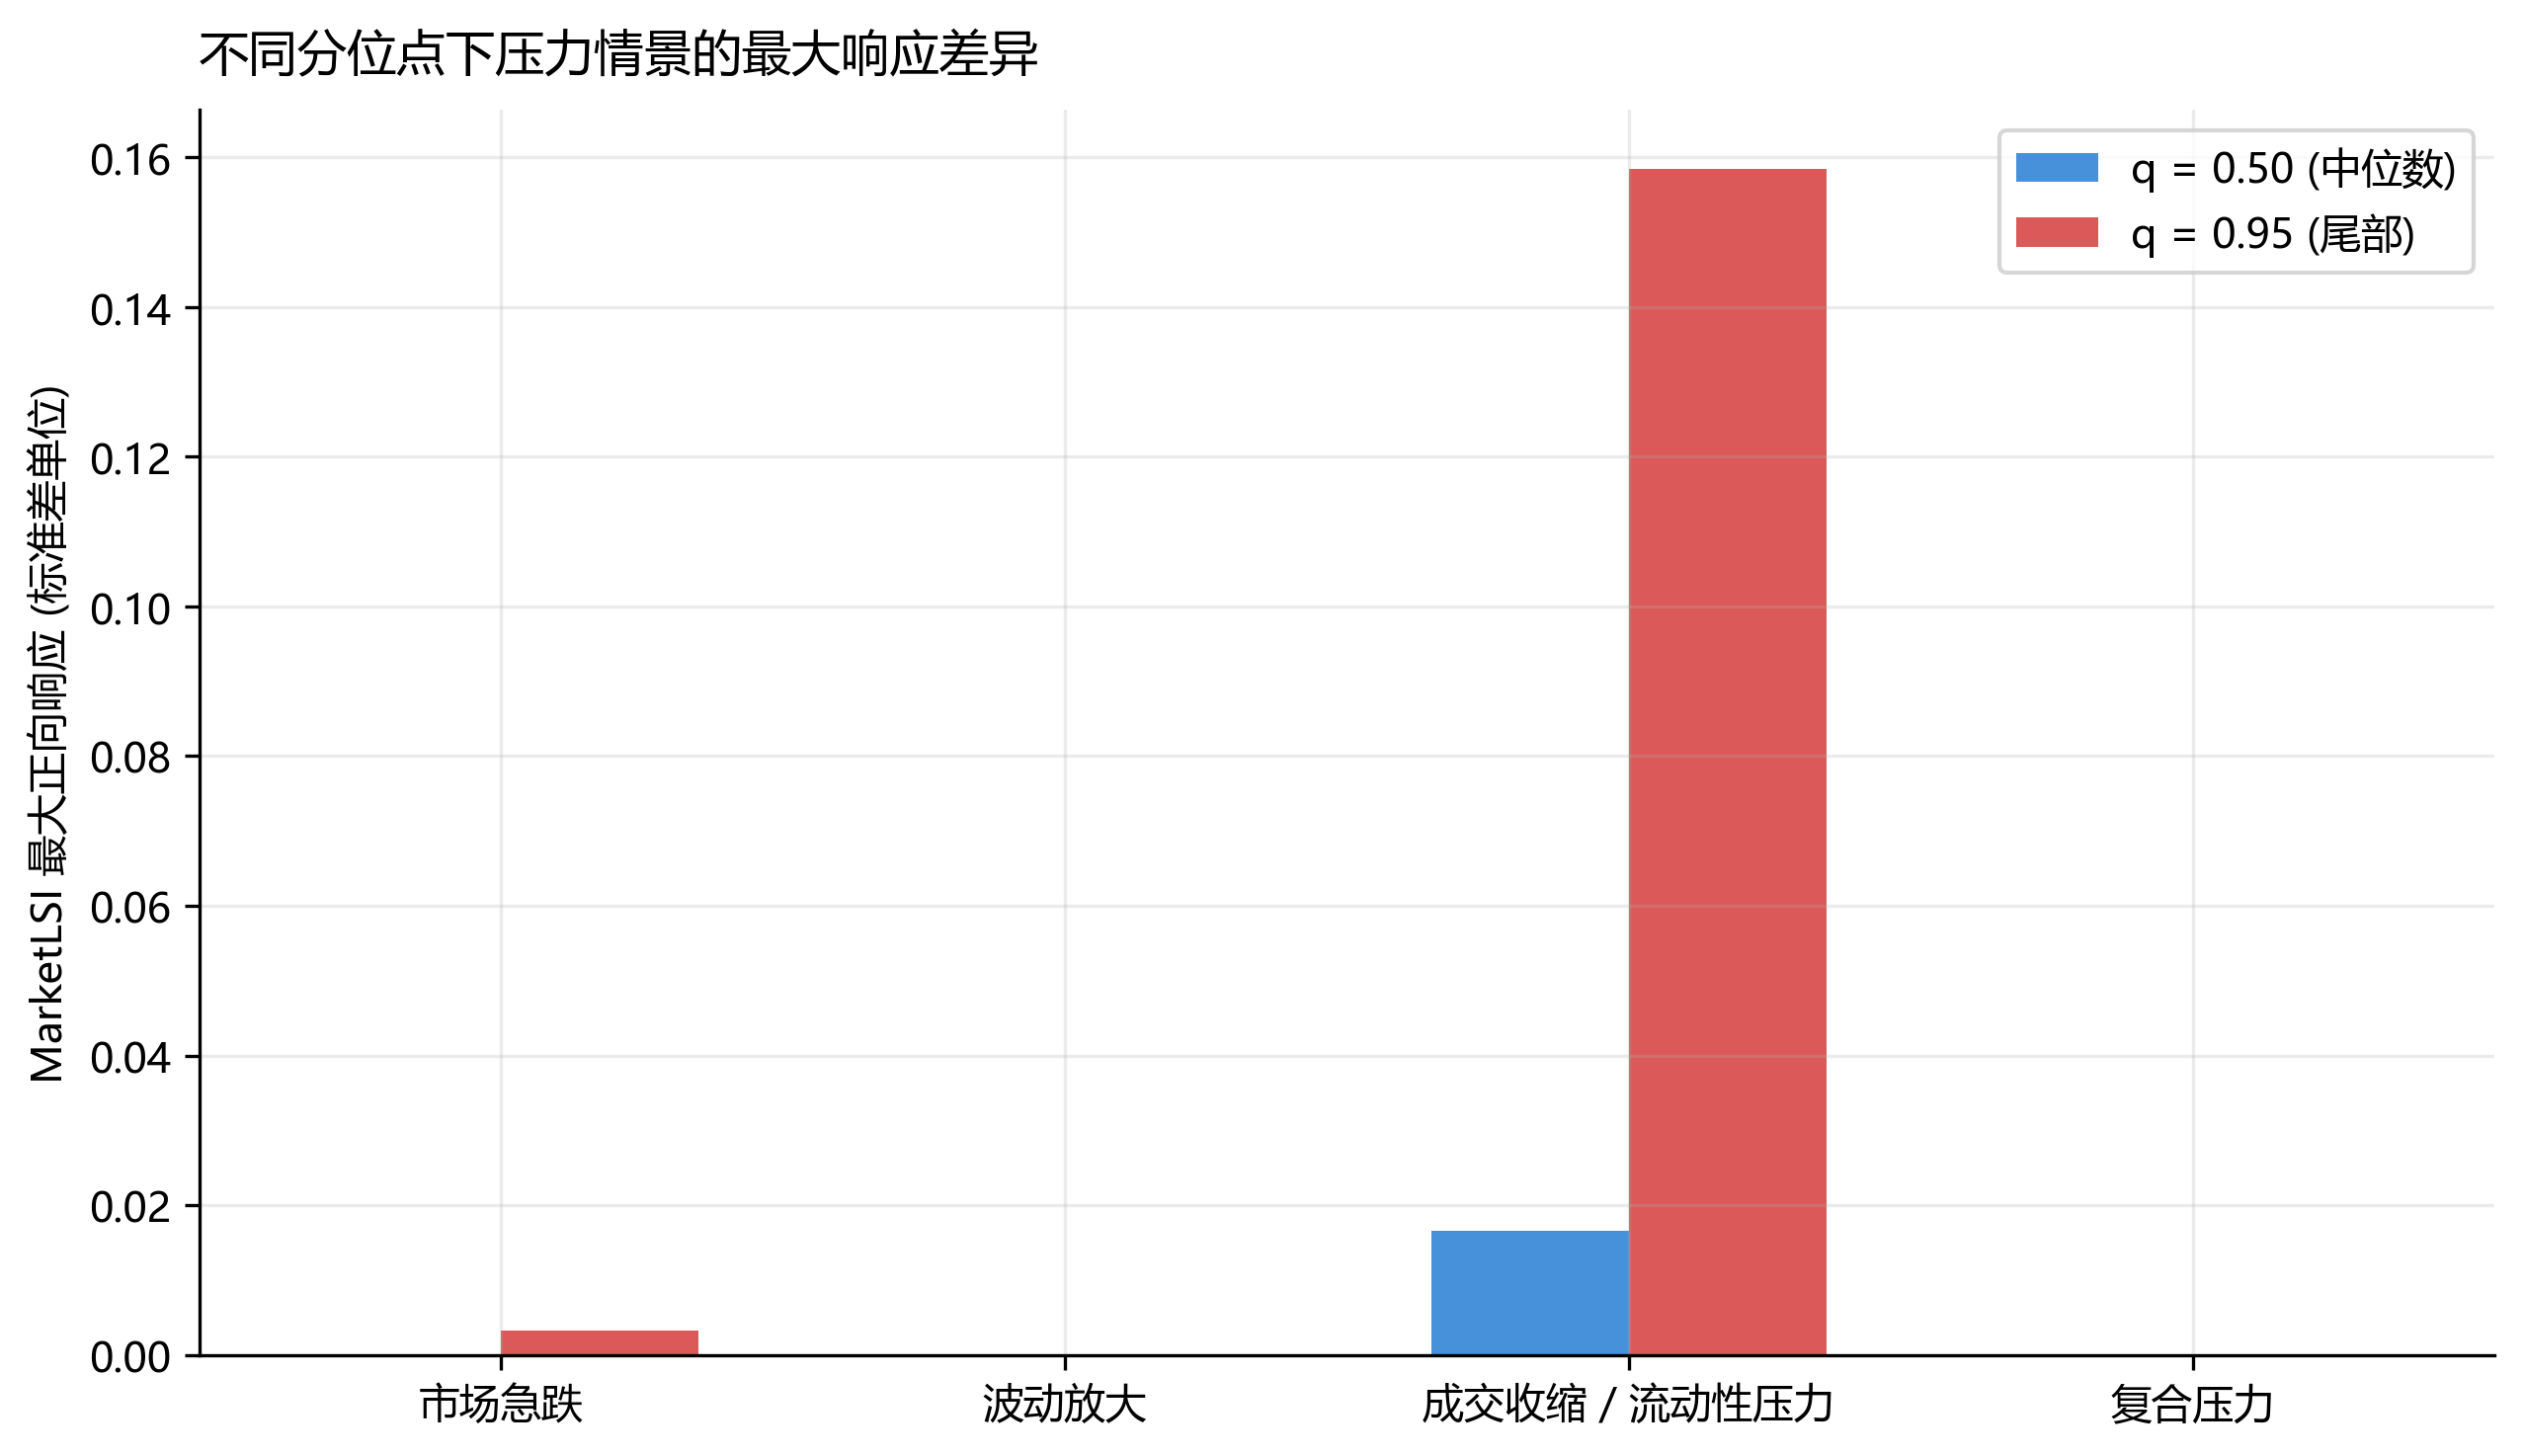
\includegraphics[width=0.86\textwidth]{figures/fig_qvar_tail_response_summary_refined.png}
    \caption{不同分位点下压力情景的最大响应差异。图中比较 \(q=0.50\) 中位数状态与 \(q=0.95\) 尾部状态下的响应强度。}
    \label{fig:qvar-tail-summary}
\end{figure}

图 \ref{fig:qvar-tail-summary} 表明，尾部分位下的响应路径与中位数状态并不完全一致，响应强度主要集中在波动放大、成交收缩或复合压力等状态下。部分情景的差异较小，说明 QVAR 稳健性证据应解释为”尾部状态下存在响应路径差异”，而不是所有情景都具有同等强度的变化。尾部分位差异主要在波动放大或复合压力等特定情景下集中体现，因此 QVAR 结果宜作为条件联动证据加以理解，而不宜无条件地推广至所有市场状态。

\subsection{SMARTBoost 特征组与 Top-K 稳健性}

对于预警模型而言，关键问题不仅是平均预测误差是否较低，更是模型能否在最高风险样本中集中识别未来压力事件。因此，本文进一步考察从 Top 1\%、Top 5\%、Top 10\% 到 Top 20\% 不同宽度高风险分组的真实压力发生率和 lift。

图 \ref{fig:robust-topk} 展示不同高风险分组下的真实压力发生率与 lift。

\begin{figure}[H]
    \centering
    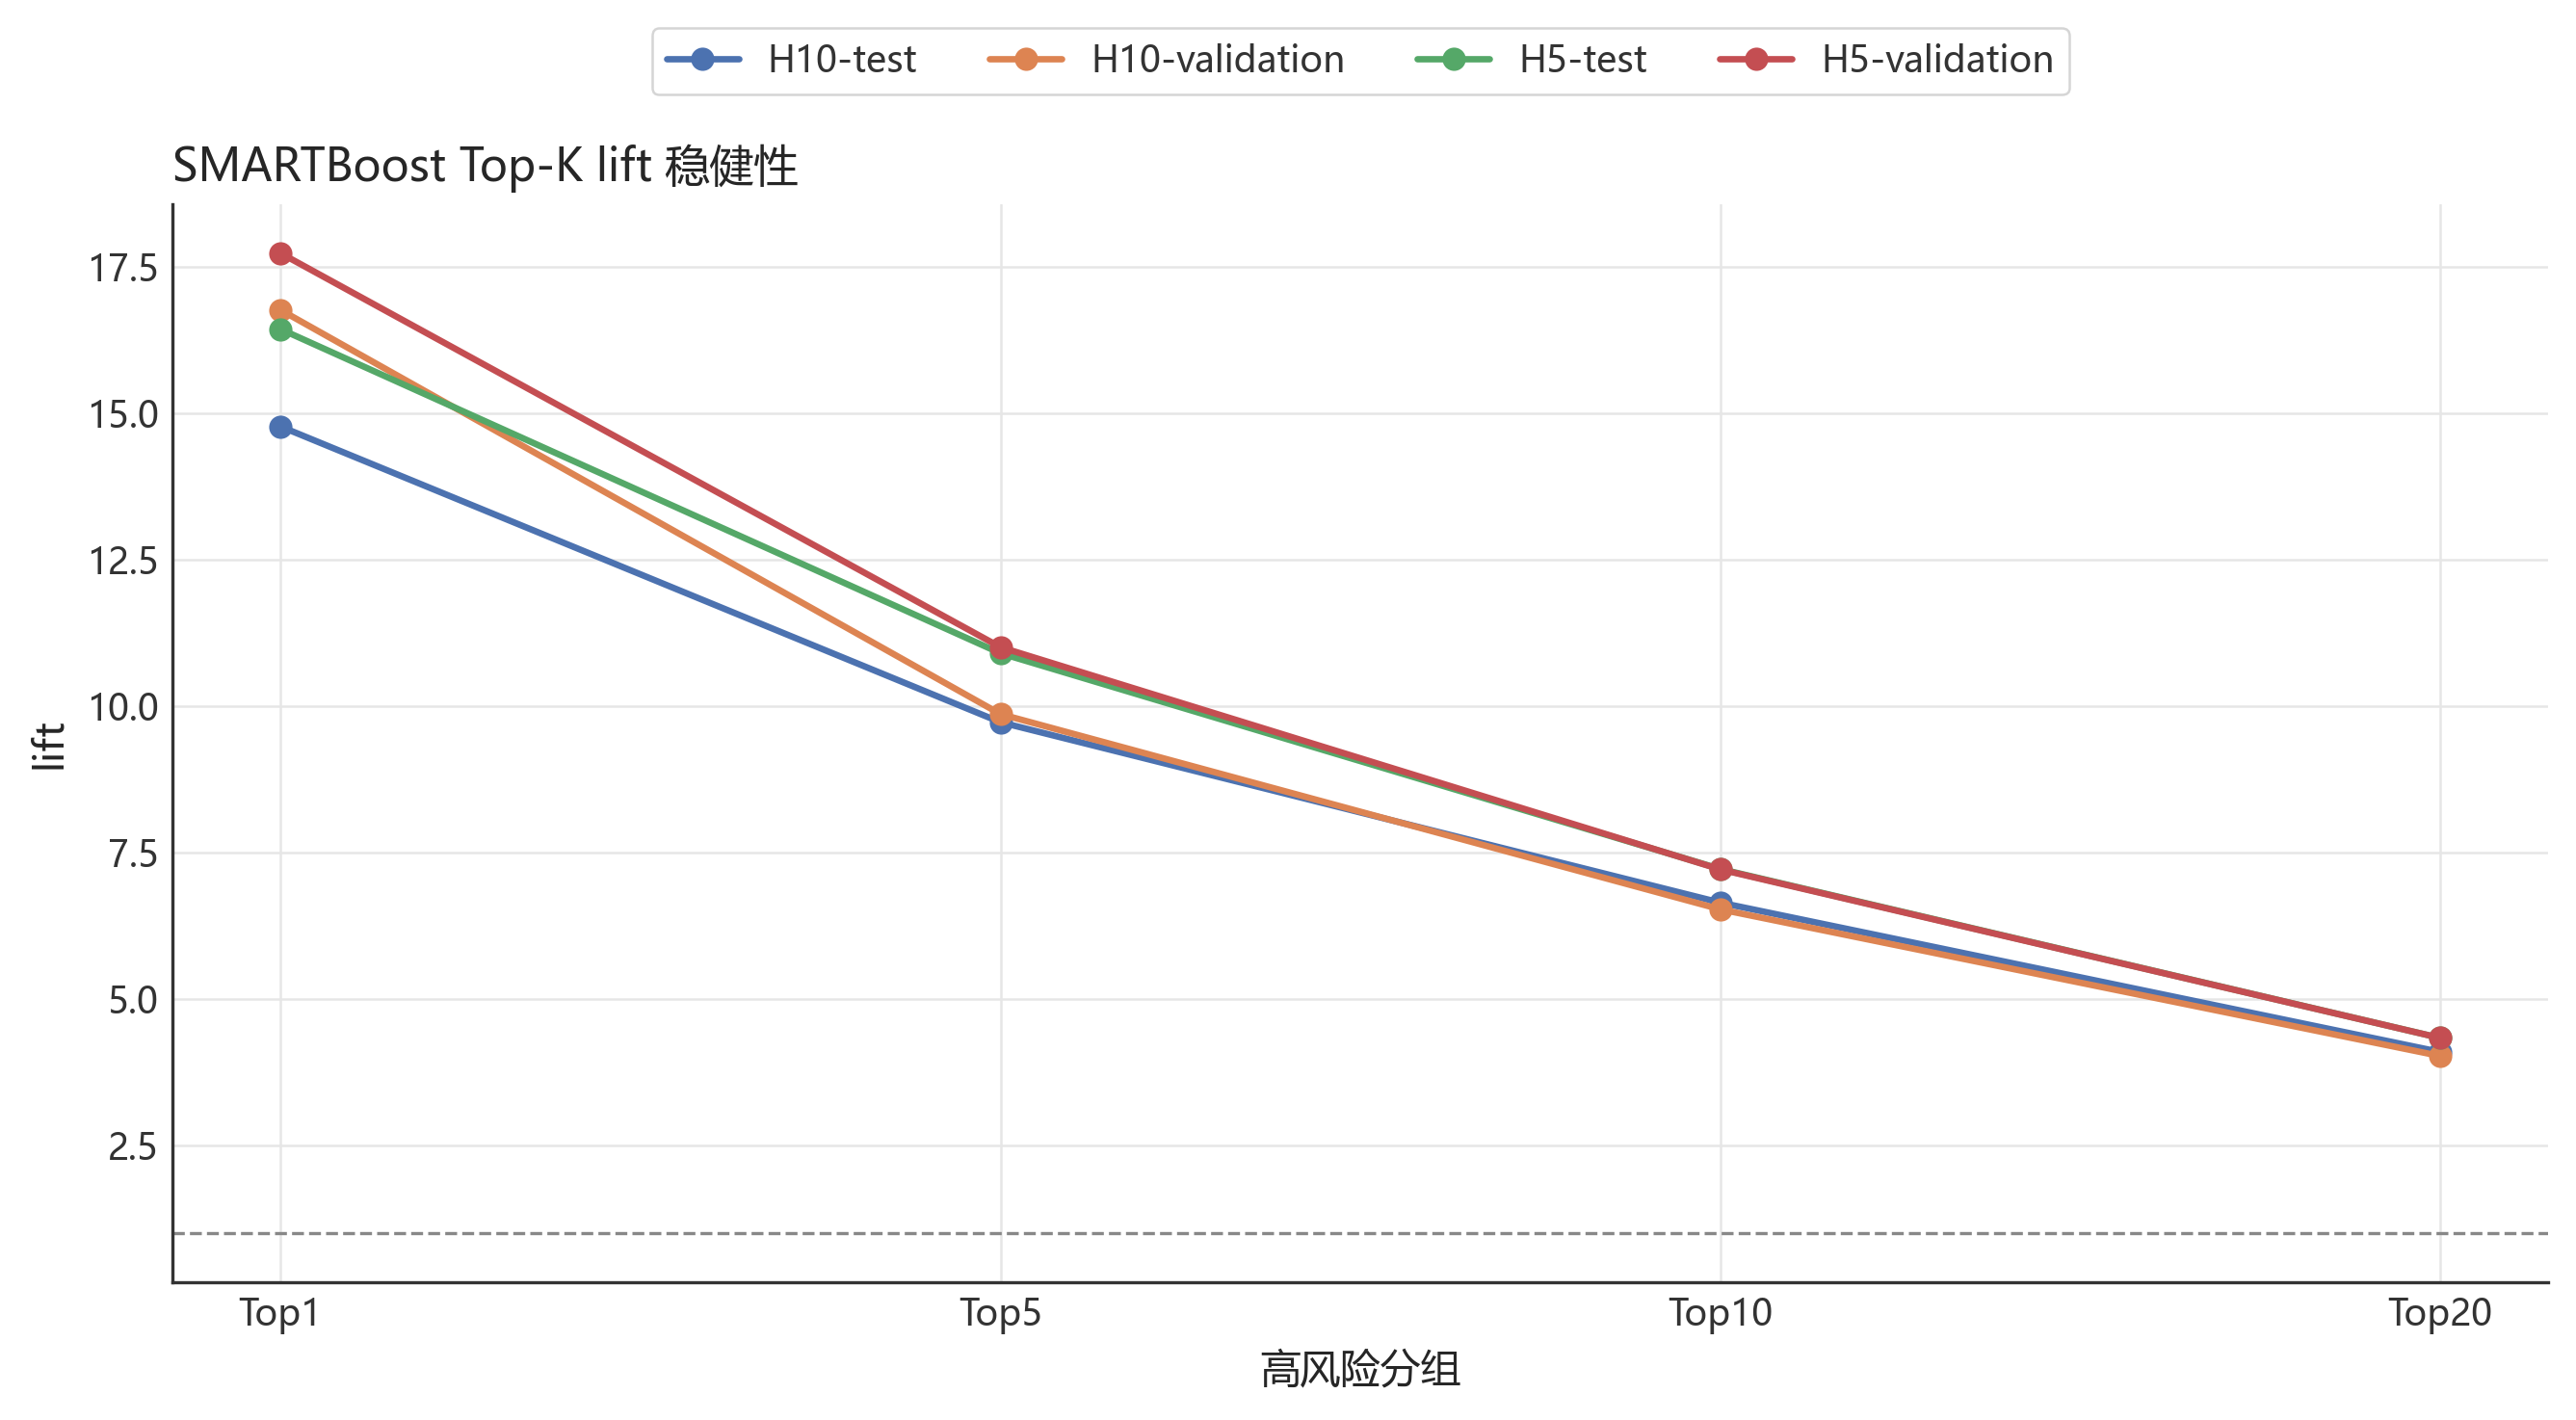
\includegraphics[width=0.90\textwidth]{figures/fig_robust_sb_topk.png}
    \caption{不同高风险分组下的真实压力发生率与 lift。图中考察 Top-K 分组扩展对预警集中度的影响。}
    \label{fig:robust-topk}
\end{figure}

图 \ref{fig:robust-topk} 显示，随着高风险分组从 Top 1\% 扩展到 Top 20\%，真实压力发生率和 lift 逐步下降，但仍高于整体事件基准率。lift 递减是合理现象，因为分组扩大必然纳入更多中等风险样本；这并不表示模型失效，而是风险排序模型的预期表现。最高风险分组具有最高事件集中度，较宽的高风险分组则提供更稳定但更温和的预警覆盖。Top-K 扩大时 lift 自然下降，但只要各分组的真实压力发生率仍高于样本整体事件率，即说明模型的排序能力并非单一阈值下的偶然结果，而具有跨分组的稳健性。

\subsection{防泄漏核查}

本文最后进行特征边界核查。核心原则是：所有进入 SMARTBoost 的特征必须在 \(t\) 时点或 \(t\) 时点以前可得，不得使用未来窗口内的 LSI、未来压力标签或由未来标签聚合得到的变量。表 \ref{tab:smartboost-leakage} 总结最终预测特征边界。

\begin{table}[H]
\centering
\caption{SMARTBoost 特征边界核查}
\label{tab:smartboost-leakage}
\small
\begin{threeparttable}
\begin{tabularx}{\textwidth}{p{0.22\textwidth}p{0.18\textwidth}Y}
\toprule
边界项 & 处理 & 说明 \\
\midrule
CrossStress & 排除 & 由未来压力标签横截面聚合得到，只可用于状态描述，不进入预测特征矩阵。 \\
压力标签 & 仅作目标变量 & Stress\_H5 与 Stress\_H10 不作为解释变量。 \\
FutureMaxLSI & 排除 & 未来窗口派生变量不进入预测特征矩阵。 \\
滚动特征 & 历史可观测 & 仅使用 \(t\) 时点及以前的信息。 \\
样本切分 & 时间顺序 & 训练、验证、测试按日期划分，不随机打乱。 \\
\bottomrule
\end{tabularx}
\begin{tablenotes}[flushleft]
\footnotesize
\item 注：本表用于说明预测特征的时间边界，避免未来窗口信息进入 SMARTBoost。
\end{tablenotes}
\end{threeparttable}
\end{table}


根据这一边界，Stress\_H5、Stress\_H10、FutureMaxLSI 以及由未来标签横截面聚合得到的 CrossStress 均被排除在最终预测特征矩阵之外。训练、验证与测试样本保持严格的时间顺序切分，标准化参数和标签阈值均仅来自训练期历史分布。因此，SMARTBoost 的样本外表现可以解释为历史高频状态变量的预警能力，而不是未来标签信息进入特征矩阵后的前视偏差。

\begin{table}[H]
\centering
\caption{稳健性检验设计}
\label{tab:robustness-design}
\small
\begin{threeparttable}
\begin{tabularx}{\textwidth}{p{0.22\textwidth}p{0.30\textwidth}Y}
\toprule
检验方向 & 替代设定 & 目的 \\
\midrule
标签阈值 & 85\% / 90\% / 95\% & 检查压力事件定义是否依赖单一训练期分位阈值。 \\
RGARCH 测度 & RV、RBV、MedRV、RMAD & 比较不同 realized pressure measure 下的拟合和样本外损失。 \\
QVAR 分位点 & 0.10 / 0.50 / 0.90 / 0.95 & 检查尾部状态和中位数状态下响应路径是否一致。 \\
SMARTBoost 特征 & 完整无泄漏特征与特征组删减 & 检查市场共同状态变量对样本外预警的增量贡献。 \\
\bottomrule
\end{tabularx}
\begin{tablenotes}[flushleft]
\footnotesize
\item 注：所有稳健性设定均保持时间顺序切分和训练期标准化边界。
\end{tablenotes}
\end{threeparttable}
\end{table}

\begin{table}[H]
\centering
\caption{稳健性检验核心结论}
\label{tab:robustness-conclusions}
\small
\begin{threeparttable}
\begin{tabularx}{\textwidth}{p{0.24\textwidth}Y p{0.18\textwidth}}
\toprule
检验方向 & 核心结果 & 结论 \\
\midrule
标签阈值 & Top 5\% lift 在 H5/H10 中保持明显高于基准事件率。 & 方向稳健 \\
RGARCH 测度 & RMAD 的 test R2LOG 为 0.030，但解释需结合测度尺度。 & 谨慎解读 \\
QVAR 分位点 & MarketLSI 在 q=0.95 的 test pinball loss 为 0.0231，尾部响应不同于中位数关系。 & 尾部差异存在 \\
SMARTBoost 特征组 & 排除 CrossStress 后仍保持样本外识别力，市场共同状态变量具有增量信息。 & 未发现未来信息泄漏 \\
\bottomrule
\end{tabularx}
\begin{tablenotes}[flushleft]
\footnotesize
\item 注：本表只报告核心方向，详细数值保留在附表材料中。
\end{tablenotes}
\end{threeparttable}
\end{table}


表 \ref{tab:robustness-design} 与表 \ref{tab:robustness-conclusions} 对本章稳健性检验进行汇总。总体来看，标签阈值、realized pressure measure、QVAR 分位点和 Top-K 预警宽度的替代设定不会改变本文的核心判断：短时压力状态具有可度量的动态结构和尾部联动特征，历史分钟级状态变量能够在样本外形成有效的高风险排序。

\FloatBarrier
